\documentclass[12pt,twoside,slovak,a4paper]{coursepaper}

\usepackage[slovak]{babel}%\usepackage[T1]{fontenc}
\usepackage[utf8]{inputenc}
\usepackage{graphicx}
\usepackage{url} % príkaz \url na formátovanie URL
\usepackage{hyperref} % odkazy v texte budú aktívne (pri niektorých triedach dokumentov spôsobuje posun textu)

\usepackage{cite}
%\usepackage{times}

\pagestyle{headings}

\title{Ensuring Data Integrity and Reliability in Big Data: A Comprehensive Study on Data Quality Management Strategies\thanks{Semestrálny projekt v predmete Metódy inžinierskej práce, ak. rok 2023/24, vedenie: Mirwais Ahmadzai}} % meno a priezvisko vyučujúceho na cvičeniach

\author{Michal Zrutta\\[2pt]
	{\small Slovenská technická univerzita v Bratislave}\\
	{\small Fakulta informatiky a informačných technológií}\\
	{\small \textt{xzrutta@stuba.sk}}
	}

\date{\small 10.october 2023} % upravte

\begin{document}

\maketitle

\begin{abstract}
We live in the era of Big Data. By looking at the statistics of globally generated data annually, we can 
see the increasing trend. If we compare the year 2010 and 2022 it shows us a difference of 95
zettabytes generated in a single year. However, the upward trajectory poses challenges in data 
quality. Consequently, the demand for realistic data sets, accurate and consistent information, and 
overall data quality has become a pressing concern. The paper aims to investigate the challenges 
related to testing in the context of Big Data adoption. It seeks to outline a testing strategy that can 
effectively validate the high volume, velocity, and variety of information associated with Big Data.\cite{gudivada2015big}\cite{mittal2013trustworthiness}
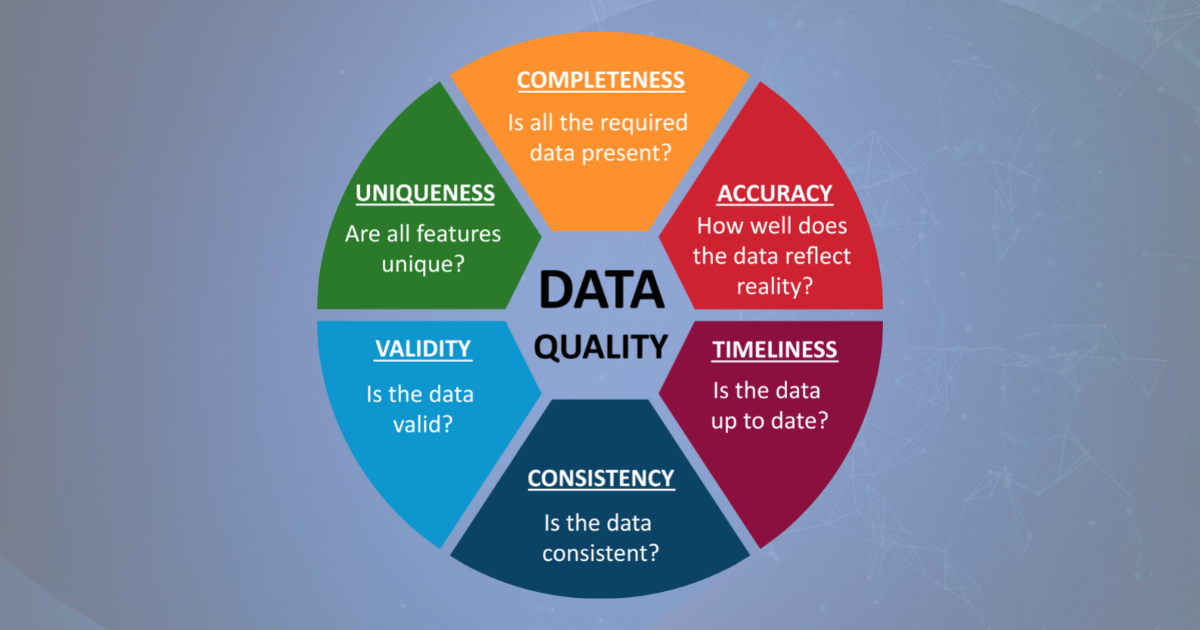
\includegraphics[scale=0.25]{../1_UUqMUEVRtKnx_mx0k1sf1Q.png}
\end{abstract} 
\bibliographystyle{abbrv}
\bibliography{citations}
\end{document}